\documentclass[12pt,final]{amsart}%default 10pt
%prepared in AMSLaTeX, under LaTeX2e

\usepackage[margin=1in]{geometry}

\usepackage{natbib}

\usepackage{amssymb,alltt,verbatim,xspace,fancyvrb}
\usepackage{palatino}

% check if we are compiling under latex or pdflatex
\ifx\pdftexversion\undefined
  \usepackage[final,dvips]{graphicx}
\else
  \usepackage[final,pdftex]{graphicx}
\fi

% hyperref should be the last package we load
\usepackage[pdftex,
                colorlinks=true,
                plainpages=false, % only if colorlinks=true
                linkcolor=blue,   % only if colorlinks=true
                citecolor=black,   % only if colorlinks=true
                urlcolor=magenta     % only if colorlinks=true
]{hyperref}

\newcommand{\normalspacing}{\renewcommand{\baselinestretch}{1.1}\tiny\normalsize}
\newcommand{\tablespacing}{\renewcommand{\baselinestretch}{1.0}\tiny\normalsize}
\normalspacing

% math macros
\newcommand\bv{\mathbf{v}}
\newcommand\bq{\mathbf{q}}

\newcommand\CC{\mathbb{C}}
\newcommand{\DDt}[1]{\ensuremath{\frac{d #1}{d t}}}
\newcommand{\ddt}[1]{\ensuremath{\frac{\partial #1}{\partial t}}}
\newcommand{\ddx}[1]{\ensuremath{\frac{\partial #1}{\partial x}}}
\newcommand{\ddy}[1]{\ensuremath{\frac{\partial #1}{\partial y}}}
\newcommand{\ddxp}[1]{\ensuremath{\frac{\partial #1}{\partial x'}}}
\newcommand{\ddz}[1]{\ensuremath{\frac{\partial #1}{\partial z}}}
\newcommand{\ddxx}[1]{\ensuremath{\frac{\partial^2 #1}{\partial x^2}}}
\newcommand{\ddyy}[1]{\ensuremath{\frac{\partial^2 #1}{\partial y^2}}}
\newcommand{\ddxy}[1]{\ensuremath{\frac{\partial^2 #1}{\partial x \partial y}}}
\newcommand{\ddzz}[1]{\ensuremath{\frac{\partial^2 #1}{\partial z^2}}}
\newcommand{\Div}{\nabla\cdot}
\newcommand\eps{\epsilon}
\newcommand{\grad}{\nabla}
\newcommand{\ihat}{\mathbf{i}}
\newcommand{\ip}[2]{\ensuremath{\left<#1,#2\right>}}
\newcommand{\jhat}{\mathbf{j}}
\newcommand{\khat}{\mathbf{k}}
\newcommand{\nhat}{\mathbf{n}}
\newcommand\lam{\lambda}
\newcommand\lap{\triangle}
\newcommand\Matlab{\textsc{Matlab}\xspace}
\newcommand\RR{\mathbb{R}}
\newcommand\vf{\varphi}

\newcommand{\Wlij}{W^l_{i,j}}
\newcommand{\Wij}{W_{i,j}}
\newcommand{\upp}[3]{\big<#1\big|_{#3}\,#2\big>}



\title[]{HYDROLAKES:  a minimal model of subglacial hydrology}

\author[]{Ed Bueler}


\begin{document}

\maketitle

\thispagestyle{empty}

%\setcounter{tocdepth}{1}
%\tableofcontents

\section{Introduction}

Any reasonable model of the aquifer has at least these two elements: liquid water is conserved and water flows from high to low hydraulic potential (``head'').  Physical processes control the geometry of the aquifer/layer (e.g.~cavities open by sliding, cavities/channels close by creep, channels open by melting, sediment moves, \dots), but we do not model these here.  Instead we model water pressure by the highly-simplified assumption that the water pressure is equal to the overburden pressure, or is a fixed multiple thereof.\footnote{This project is a fork from the project that Sarah Child and Brad Booch did at the 2nd McCarthy Summer School in Glaciology in 2012.}  The assumption that water pressure is equal to the overburden pressure is justified if creep closure dominates over sliding or wall melt.


\section{Continuum model}

We consider a layer of water with thickness $W(t,x,y)$.  It is only likely to be meaningful, however, if it is regarded as an average over a horizontal scale of tens to thousands of meters.  While the hydrologic system has fine spatial variation which one is unlikely to be able to model, we will attempt only to model spatially-averaged versions of water amount and water pressure.  We assume that the water is incompressible.  Choosing to model the subglacial hydrology using a water thickness is therefore not a significant restriction on the physics, and the thickness of water tells us the mass of water.

Water is conserved, so that in two spatial dimensions it is described by the equation \citep{Clarke05}
\begin{equation} \label{eq:conserve}
W_t + \Div \bq = \Phi
\end{equation}
where $\bq$ is the vector water flux (units $\text{m}^2\,\text{s}^{-1}$) and $\Phi$ is a source term ($\text{m}\,\text{s}^{-1}$).

We might separate the water sources between the melt on the lower surface of the glacier and the en- or supra-glacial drainage origin,
  $$\Phi = \rho_w^{-1} \left(m + S\right)$$
where $\rho_w$ is the density of fresh liquid water, $m$ is the rate at which basal melting (refreeze) of ice adds (removes) water, and $S$ is the rate at which surface runoff or englacial drainage adds water.  For the first example below we will take $\Phi$ to be constant.  Note $m$ and $S$ have units $\text{kg}\,\text{m}^{-2}\,\text{s}^{-1}$.

The water flux $\bq$ in equation \eqref{eq:conserve} is related to the gradient of a hydraulic potential $\psi(t,x,y)$ which combines the actual water pressure $P(t,x,y)$ and the gravitational potential corresponding to top of the layer of water at the location on the bed of the glacier,
\begin{equation} \label{eq:potential}
\psi = P + \rho_w g\, (b+W).
\end{equation}
Here $z=b(x,y)$ is the time-independent bedrock elevation, which we assume is given by time-independent data.

Water flows from high to low hydraulic potential.  The simplest model is for a water sheet \citep{Clarke05}
\begin{equation}  \label{eq:flux}
\bq = - \frac{K \, W}{\rho_w g} \grad \psi
\end{equation}
Here, $\rho_w$ is the water density ($\text{kg}\,\text{m}^{-3}$), $g$ the gravitational acceleration ($\text{m}\,\text{s}^{-2}$) and $K$ is the effective hydraulic conductivity ($\text{m}\,\text{s}^{-1}$).  Notice that the system transmits more water for a given head gradient if either the holes through the subglacial material are bigger ($K$ is larger) or the water sheet is thicker ($W$ is larger).

Recall that the ice is a fluid which has a pressure field of its own, with basal value $P_i$, the \emph{overburden pressure}.  In this minimal model, water pressure $P$ is proportional to the ice overburden pressure.  We also make, as an acceptable shallow approximation \citep{GreveBlatter2009}, the assumption that the ice pressure is hydrostatic
\begin{equation} \label{eq:hydrostatic}
  P_i = \rho_i g H = \rho_i g (h-b).
\end{equation}
Here $\rho_i$ is the density of ice ($\text{kg}\,\text{m}^{-3}$), $H$ is the ice thickness (m), and $h$ is the ice upper surface elevation (m).  Our model for the subglacial water pressure is
\begin{equation} \label{eq:pisoverburden}
  P = s P_i
\end{equation}
where $s$ is a dimensionless constant $0\le s \le 1$.  In the case $s=1$ this model has been used for subglacial water in Antarctica \citep{LeBrocqetal2009}.

Let $r = \rho_i / \rho_w \approx 0.9$, a dimensionless constant.  From equations \eqref{eq:potential}, \eqref{eq:flux}, \eqref{eq:hydrostatic}, and \eqref{eq:pisoverburden} we derive a more transparent description of the flux,
\begin{equation} \label{eq:qexpression}
  \bq = \bv\, W - K W \grad W
\end{equation}
where
\begin{equation} \label{eq:vexpression}
  \bv = - K \left(s r \grad h + (1-sr) \grad b\right)
\end{equation}
is an ice-sheet-geometry-dependent vector function which has units of velocity.  Thus the water flow $\bq$ mostly depends on the surface and bedrock slope because the velocity $\bv$ is a sum of these slopes.  However, because the bedrock elevation comes from rough data in practice, the distribution of the velocity $\bv$ will not be very smooth.  Indeed, for $s\approx 1$ the typically-smoother surface gradient is more important, while for $s \ll 1$ the typically-rougher bedrock gradient becomes more significant.

From equations \eqref{eq:conserve} and \eqref{eq:qexpression} we derive an advection-diffusion equation \citep{HundsdorferVerwer2010,MortonMayers},
\begin{equation} \label{eq:adeqn}
  W_t + \Div\left(\bv\, W\right) = \Div \left(K W \grad W\right) + \Phi
\end{equation}


\section{Numerical scheme}

Equation \eqref{eq:adeqn} is discretized by an explicit\footnote{This is a first draft.  I expect to find that ``explicit'' is not good enough because on fine grids the diffusive time-step restriction is too severe.  The most natural ``good enough'' guess for a scheme is a semi-implicit solution with implicit treatment of the diffusive part.} conservative first-order upwind method for the advection part and a centered, second-order scheme for the nonlinear diffusion part.  To set notation, suppose our rectangular computational domain has $M_x \times M_y$ gridpoints $(x_i,y_j)$ with uniform spacing $\Delta x,\Delta y$.  Let $\Wlij \approx W(t_l,x_i,y_j)$ be the approximation of the continuum solution at the grid point.

To explain the upwind method, consider the model equation
\begin{equation} \label{eq:modeladvect}
u_t + (v(x) u)_x = 0
\end{equation}
for some quantity $u(t,x)$ transported by a flux $q = v(x) u$.  We describe our ``donor cell'' upwind scheme as a finite volume scheme \citep{LeVeque} wherein a grid point $x_j$ is the center of a cell.  We consider the flux at the interfaces $x_{j-1/2}$ and $x_{j+1/2}$.  We decide which spatial finite difference to compute based on the sign of the velocity $v(x)$ at the interfaces between cells.  The scheme is easier to display if we define the following upwind notation,
\newcommand{\up}[2]{\big<#1\big|\,#2\big>}
	$$\up{v}{U_j} := v \begin{Bmatrix} U_j, & v \ge 0 \\ U_{j+1}, & v < 0 \end{Bmatrix}.$$
For the model equation \eqref{eq:modeladvect} on a space-time grid $(t_l,x_j)$ we set
\begin{equation}\label{eq:modelfdadvect}
\frac{U_j^{l+1} - U_j^l}{\Delta t} + \frac{\up{v_+}{U_j^l} - \up{v_-}{U_{j-1}^l}}{\Delta x} = 0
\end{equation}
where $v_+ = v(x_{j+1/2})$ and $v_-=v(x_{j-1/2})$.

Now we can state our scheme for equation \eqref{eq:adeqn}.  Suppose the velocity has components $\bv = (\alpha,\beta)$ and recall that $\Div \left(\bv W\right) = (\alpha W)_x + (\beta W)_y$.  We will compute velocity components at staggered (cell-face-centered) points, shown with triangle markers in Figure \ref{fig:stencil}, and use ``compass'' notation for the components: $\alpha_e = \alpha_{i+1/2,j}$, $\alpha_w = \alpha_{i-1/2,j}$, $\beta_n = \beta_{i,j+1/2}$, $\beta_s = \beta_{i,j-1/2}$.  Similarly for the diffusive term, the averages of the current water thicknesses, again computed on the staggered grid points, are denoted as follows: $W_e = (W_{i,j}^l + W_{i+1,j}^l)/2$, $W_w = (W_{i-1,j}^l + W_{i,j}^l)/2$, $W_n = (W_{i,j}^l + W_{i,j+1}^l)/2$, $W_s = (W_{i,j-1}^l + W_{i,j}^l)/2$.

\begin{figure}[ht]
\centering
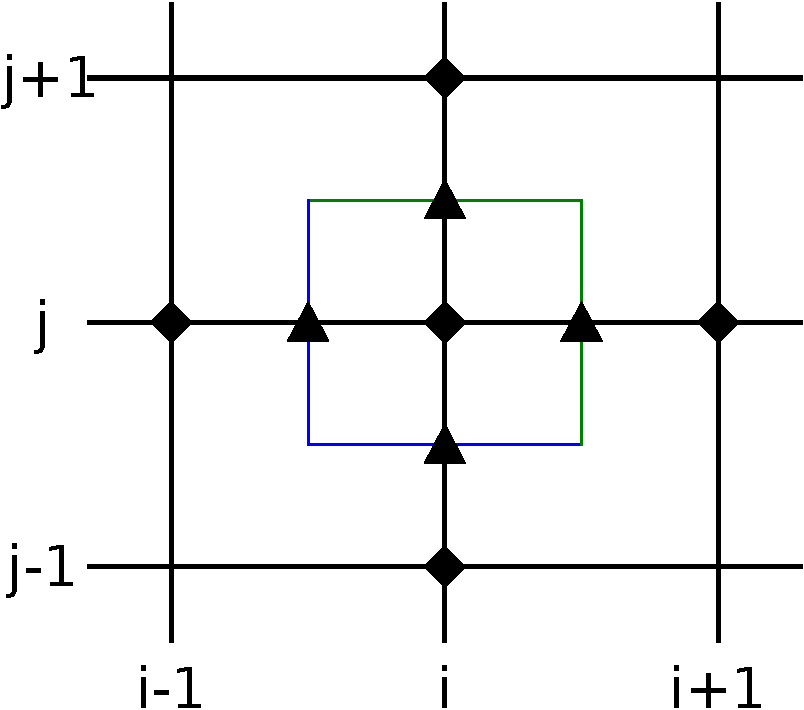
\includegraphics[width=2.5in,keepaspectratio=true]{diffstencil}
\bigskip
\caption{Numerical scheme \eqref{eq:Wfd} for Equation \eqref{eq:adeqn} computes velocity components $\bv=(\alpha,\beta)$, and averaged current water thicknesses $W$ at the staggered grid locations shown with triangles.  The finite volume scheme is a donor-cell first-order upwind method for the dashed cell.}
\label{fig:stencil}
\end{figure}

We apply the conservative upwind scheme in each variable, indicating the active index (either $i$ or $j$) in our upwind notation:
\begin{align}
 &\frac{W_{i,j}^{l+1} - \Wlij}{\Delta t} + \frac{\upp{\alpha_e}{\Wlij}{i} - \upp{\alpha_w}{W_{i-1,j}^l}{i}}{\Delta x} + \frac{\upp{\beta_n}{\Wlij}{j} - \upp{\beta_s}{W_{i,j-1}^l}{j}}{\Delta y}  \label{eq:Wfd} \\
      &\qquad = K \bigg[\frac{W_e \left(W_{i+1,j}^l - \Wlij\right) - W_w \left(\Wlij - W_{i-1,j}^l\right)}{\Delta x^2}  \notag \\
      &\qquad\qquad\qquad + \frac{W_n \left(W_{i,j+1}^l - \Wlij\right) - W_s \left(\Wlij - W_{i,j-1}^l\right)}{\Delta y^2}\bigg] + \Phi_{ij}. \notag
\end{align}
Because of the first-order upwinding this scheme has $O(\Delta t^1 + \Delta x^1 + \Delta y^1)$ truncation error.




\small
\bibliography{ice_bib}  % generally requires link to pism/doc/ice_bib.bib
\bibliographystyle{agu}


\end{document}
